\documentclass[twoside]{book}

% Packages required by doxygen
\usepackage{calc}
\usepackage{doxygen}
\usepackage{graphicx}
\usepackage[utf8]{inputenc}
\usepackage{makeidx}
\usepackage{multicol}
\usepackage{multirow}
\usepackage{textcomp}
\usepackage[table]{xcolor}

% Font selection
\usepackage[T1]{fontenc}
\usepackage{mathptmx}
\usepackage[scaled=.90]{helvet}
\usepackage{courier}
\usepackage{amssymb}
\usepackage{sectsty}
\renewcommand{\familydefault}{\sfdefault}
\allsectionsfont{%
  \fontseries{bc}\selectfont%
  \color{darkgray}%
}
\renewcommand{\DoxyLabelFont}{%
  \fontseries{bc}\selectfont%
  \color{darkgray}%
}

% Page & text layout
\usepackage{geometry}
\geometry{%
  a4paper,%
  top=2.5cm,%
  bottom=2.5cm,%
  left=2.5cm,%
  right=2.5cm%
}
\tolerance=750
\hfuzz=15pt
\hbadness=750
\setlength{\emergencystretch}{15pt}
\setlength{\parindent}{0cm}
\setlength{\parskip}{0.2cm}
\makeatletter
\renewcommand{\paragraph}{%
  \@startsection{paragraph}{4}{0ex}{-1.0ex}{1.0ex}{%
    \normalfont\normalsize\bfseries\SS@parafont%
  }%
}
\renewcommand{\subparagraph}{%
  \@startsection{subparagraph}{5}{0ex}{-1.0ex}{1.0ex}{%
    \normalfont\normalsize\bfseries\SS@subparafont%
  }%
}
\makeatother

% Headers & footers
\usepackage{fancyhdr}
\pagestyle{fancyplain}
\fancyhead[LE]{\fancyplain{}{\bfseries\thepage}}
\fancyhead[CE]{\fancyplain{}{}}
\fancyhead[RE]{\fancyplain{}{\bfseries\leftmark}}
\fancyhead[LO]{\fancyplain{}{\bfseries\rightmark}}
\fancyhead[CO]{\fancyplain{}{}}
\fancyhead[RO]{\fancyplain{}{\bfseries\thepage}}
\fancyfoot[LE]{\fancyplain{}{}}
\fancyfoot[CE]{\fancyplain{}{}}
\fancyfoot[RE]{\fancyplain{}{\bfseries\scriptsize Generated on Mon Jul 8 2013 09:22:41 for My Project by Doxygen }}
\fancyfoot[LO]{\fancyplain{}{\bfseries\scriptsize Generated on Mon Jul 8 2013 09:22:41 for My Project by Doxygen }}
\fancyfoot[CO]{\fancyplain{}{}}
\fancyfoot[RO]{\fancyplain{}{}}
\renewcommand{\footrulewidth}{0.4pt}
\renewcommand{\chaptermark}[1]{%
  \markboth{#1}{}%
}
\renewcommand{\sectionmark}[1]{%
  \markright{\thesection\ #1}%
}

% Indices & bibliography
\usepackage{natbib}
\usepackage[titles]{tocloft}
\setcounter{tocdepth}{3}
\setcounter{secnumdepth}{5}
\makeindex

% Hyperlinks (required, but should be loaded last)
\usepackage{ifpdf}
\ifpdf
  \usepackage[pdftex,pagebackref=true]{hyperref}
\else
  \usepackage[ps2pdf,pagebackref=true]{hyperref}
\fi
\hypersetup{%
  colorlinks=true,%
  linkcolor=blue,%
  citecolor=blue,%
  unicode%
}

% Custom commands
\newcommand{\clearemptydoublepage}{%
  \newpage{\pagestyle{empty}\cleardoublepage}%
}


%===== C O N T E N T S =====

\begin{document}

% Titlepage & ToC
\hypersetup{pageanchor=false}
\pagenumbering{roman}
\begin{titlepage}
\vspace*{7cm}
\begin{center}%
{\Large My Project }\\
\vspace*{1cm}
{\large Generated by Doxygen 1.8.4}\\
\vspace*{0.5cm}
{\small Mon Jul 8 2013 09:22:41}\\
\end{center}
\end{titlepage}
\clearemptydoublepage
\tableofcontents
\clearemptydoublepage
\pagenumbering{arabic}
\hypersetup{pageanchor=true}

%--- Begin generated contents ---
\chapter{Sudoku}
\label{md_README}
\hypertarget{md_README}{}
P\-R\-O\-Y\-E\-C\-T\-O D\-E S\-U\-D\-O\-K\-U L\-U\-I\-S V\-A\-S\-Q\-U\-E\-Z R\-U\-G\-E\-L L\-U\-I\-S C\-A\-V\-I\-E\-D\-E\-S 
\chapter{Hierarchical Index}
\section{Class Hierarchy}
This inheritance list is sorted roughly, but not completely, alphabetically\-:\begin{DoxyCompactList}
\item \contentsline{section}{Jugador}{\pageref{class_jugador}}{}
\item Q\-Dialog\begin{DoxyCompactList}
\item \contentsline{section}{acercade}{\pageref{classacercade}}{}
\item \contentsline{section}{eleccion}{\pageref{classeleccion}}{}
\item \contentsline{section}{instrucciones}{\pageref{classinstrucciones}}{}
\item \contentsline{section}{Ranking}{\pageref{class_ranking}}{}
\item \contentsline{section}{Ventana\-Principal}{\pageref{class_ventana_principal}}{}
\end{DoxyCompactList}
\item Q\-L\-C\-D\-Number\begin{DoxyCompactList}
\item \contentsline{section}{L\-C\-D\-Number}{\pageref{class_l_c_d_number}}{}
\end{DoxyCompactList}
\item Q\-Main\-Window\begin{DoxyCompactList}
\item \contentsline{section}{sudoku}{\pageref{classsudoku}}{}
\end{DoxyCompactList}
\end{DoxyCompactList}

\chapter{Class Index}
\section{Class List}
Here are the classes, structs, unions and interfaces with brief descriptions\-:\begin{DoxyCompactList}
\item\contentsline{section}{\hyperlink{classacercade}{acercade} }{\pageref{classacercade}}{}
\item\contentsline{section}{\hyperlink{classeleccion}{eleccion} }{\pageref{classeleccion}}{}
\item\contentsline{section}{\hyperlink{classinstrucciones}{instrucciones} }{\pageref{classinstrucciones}}{}
\item\contentsline{section}{\hyperlink{class_jugador}{Jugador} }{\pageref{class_jugador}}{}
\item\contentsline{section}{\hyperlink{class_l_c_d_number}{L\-C\-D\-Number} }{\pageref{class_l_c_d_number}}{}
\item\contentsline{section}{\hyperlink{class_ranking}{Ranking} }{\pageref{class_ranking}}{}
\item\contentsline{section}{\hyperlink{classsudoku}{sudoku} }{\pageref{classsudoku}}{}
\item\contentsline{section}{\hyperlink{class_ventana_principal}{Ventana\-Principal} }{\pageref{class_ventana_principal}}{}
\end{DoxyCompactList}

\chapter{File Index}
\section{File List}
Here is a list of all documented files with brief descriptions\-:\begin{DoxyCompactList}
\item\contentsline{section}{\hyperlink{acercade_8h}{acercade.\-h} \\*Contiene una descripcion sobre los creadores del juego }{\pageref{acercade_8h}}{}
\item\contentsline{section}{\hyperlink{eleccion_8h}{eleccion.\-h} \\*Este archivo contiene la definicion de los slots para el comienzo del juego }{\pageref{eleccion_8h}}{}
\item\contentsline{section}{\hyperlink{instrucciones_8h}{instrucciones.\-h} \\*Contiene una breve explicación de la jugabilidad del sudoku }{\pageref{instrucciones_8h}}{}
\item\contentsline{section}{\hyperlink{jugador_8h}{jugador.\-h} \\*Contiene la declaracion del tipo de datos jugador y sus respectivos getter y setter }{\pageref{jugador_8h}}{}
\item\contentsline{section}{\hyperlink{lcdnumber_8h}{lcdnumber.\-h} \\*Contiene la definicion del cronometro utilizado en la interfaz del sudoku }{\pageref{lcdnumber_8h}}{}
\item\contentsline{section}{\hyperlink{ranking_8h}{ranking.\-h} \\*Presentacion de los jugadores que han terminado el sudoku de manera satisfactoria }{\pageref{ranking_8h}}{}
\item\contentsline{section}{\hyperlink{sudoku_8h}{sudoku.\-h} \\*Este archivo contiene la definicion de las funciones para el la creación, validación y presentación del sudoku. ademas permite cargar y guardar la partida }{\pageref{sudoku_8h}}{}
\item\contentsline{section}{\hyperlink{ventanaprincipal_8h}{ventanaprincipal.\-h} \\*Ventana principal del juego Sudoku }{\pageref{ventanaprincipal_8h}}{}
\end{DoxyCompactList}

\chapter{Class Documentation}
\hypertarget{classacercade}{\section{acercade Class Reference}
\label{classacercade}\index{acercade@{acercade}}
}
Inheritance diagram for acercade\-:\begin{figure}[H]
\begin{center}
\leavevmode
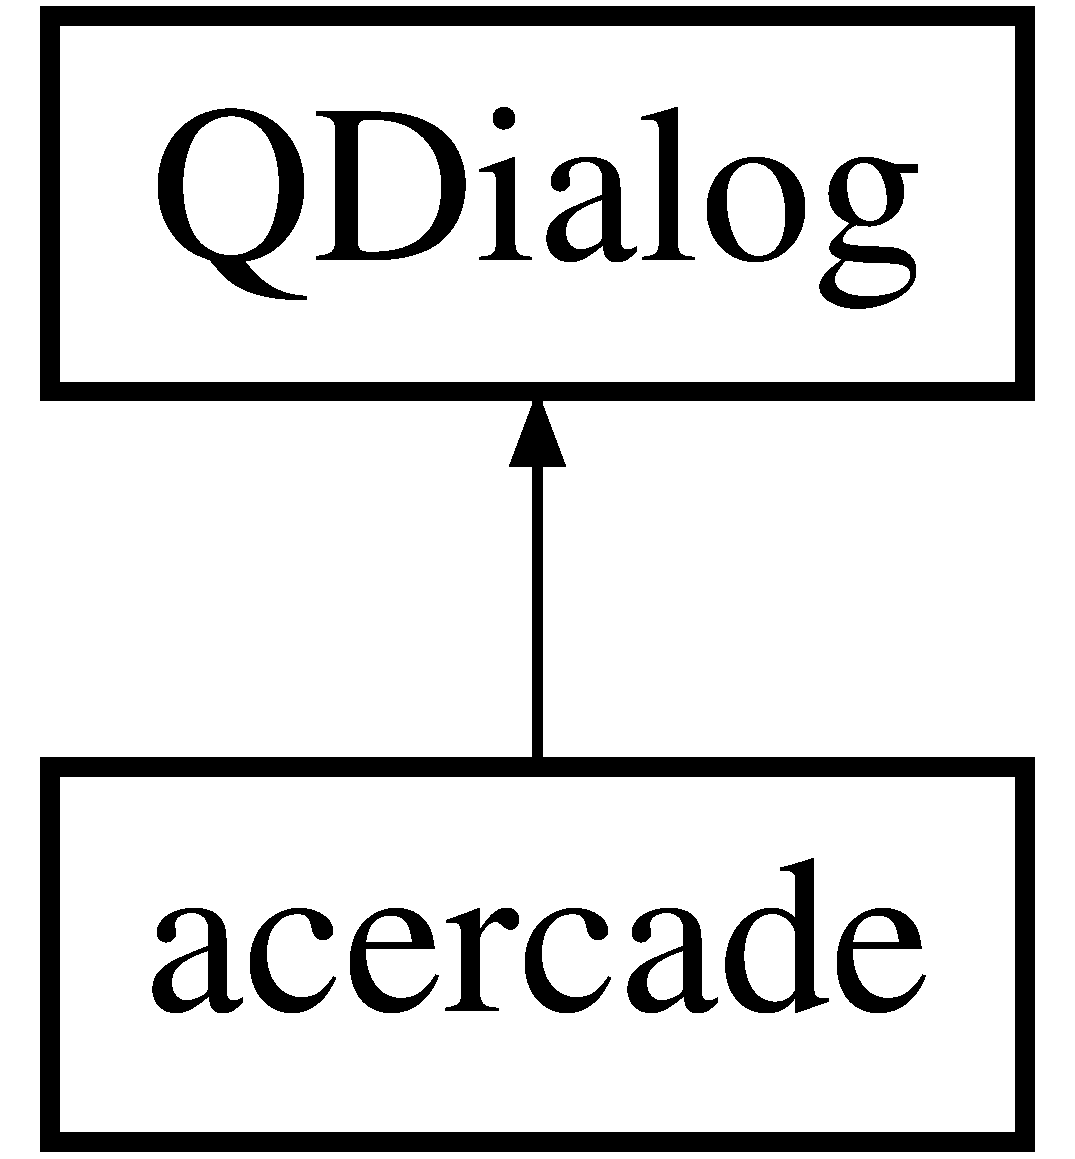
\includegraphics[height=2.000000cm]{classacercade}
\end{center}
\end{figure}
\subsection*{Public Member Functions}
\begin{DoxyCompactItemize}
\item 
\hypertarget{classacercade_abc0954c76a298550883117ede795f268}{{\bfseries acercade} (Q\-Widget $\ast$parent=0)}\label{classacercade_abc0954c76a298550883117ede795f268}

\end{DoxyCompactItemize}


The documentation for this class was generated from the following files\-:\begin{DoxyCompactItemize}
\item 
\hyperlink{acercade_8h}{acercade.\-h}\item 
acercade.\-cpp\end{DoxyCompactItemize}

\hypertarget{classeleccion}{\section{eleccion Class Reference}
\label{classeleccion}\index{eleccion@{eleccion}}
}
Inheritance diagram for eleccion\-:\begin{figure}[H]
\begin{center}
\leavevmode
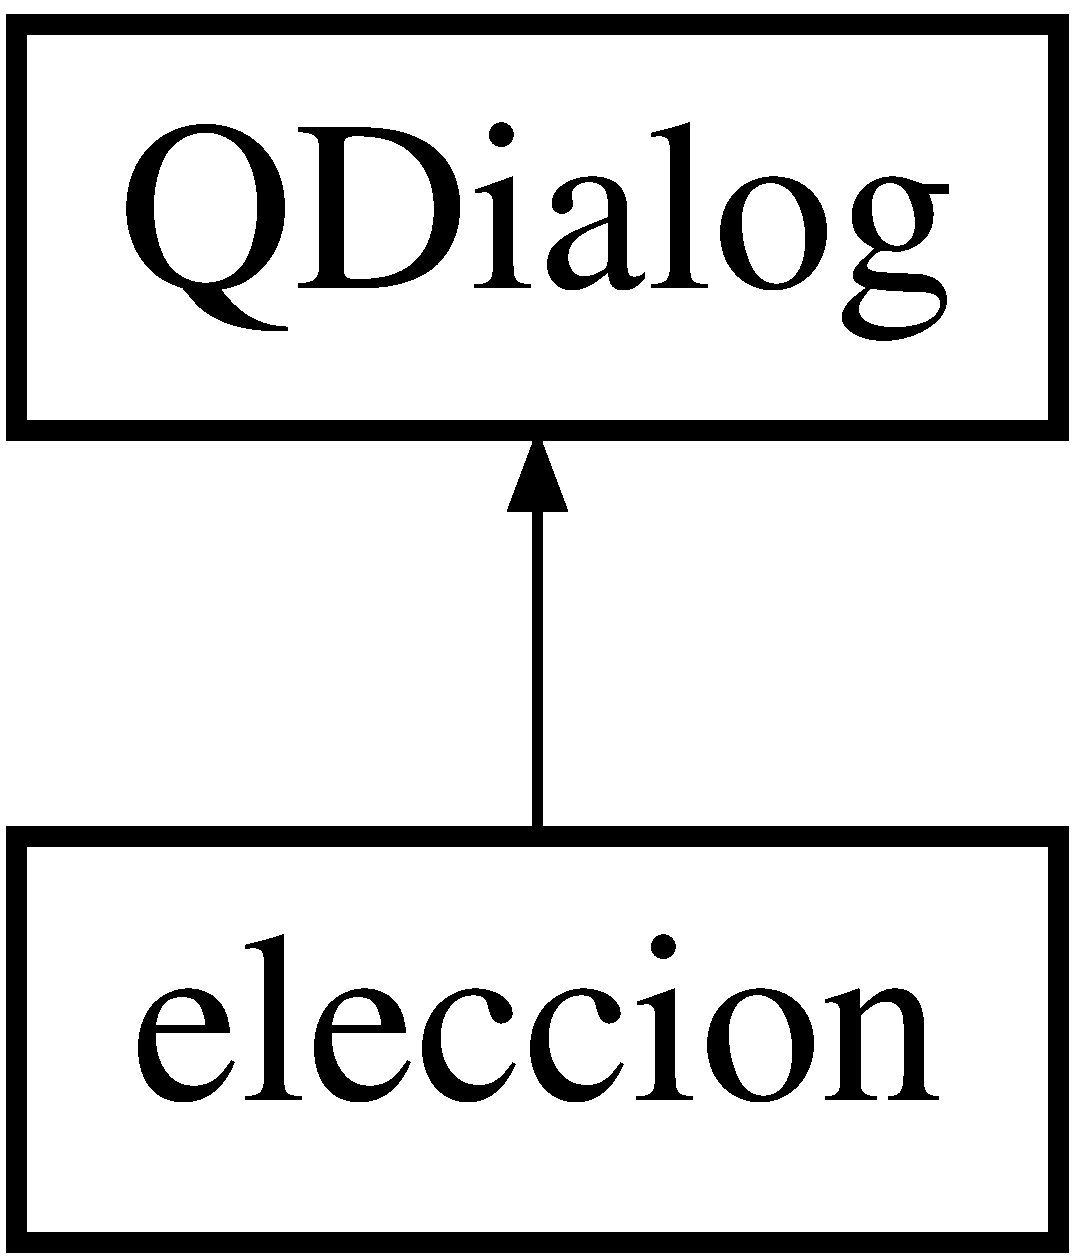
\includegraphics[height=2.000000cm]{classeleccion}
\end{center}
\end{figure}
\subsection*{Public Member Functions}
\begin{DoxyCompactItemize}
\item 
\hypertarget{classeleccion_a9d9a1b39e8e0b70e3388fbdf8f1936c7}{{\bfseries eleccion} (Q\-Widget $\ast$parent=0)}\label{classeleccion_a9d9a1b39e8e0b70e3388fbdf8f1936c7}

\end{DoxyCompactItemize}


The documentation for this class was generated from the following files\-:\begin{DoxyCompactItemize}
\item 
\hyperlink{eleccion_8h}{eleccion.\-h}\item 
eleccion.\-cpp\end{DoxyCompactItemize}

\hypertarget{classinstrucciones}{\section{instrucciones Class Reference}
\label{classinstrucciones}\index{instrucciones@{instrucciones}}
}
Inheritance diagram for instrucciones\-:\begin{figure}[H]
\begin{center}
\leavevmode
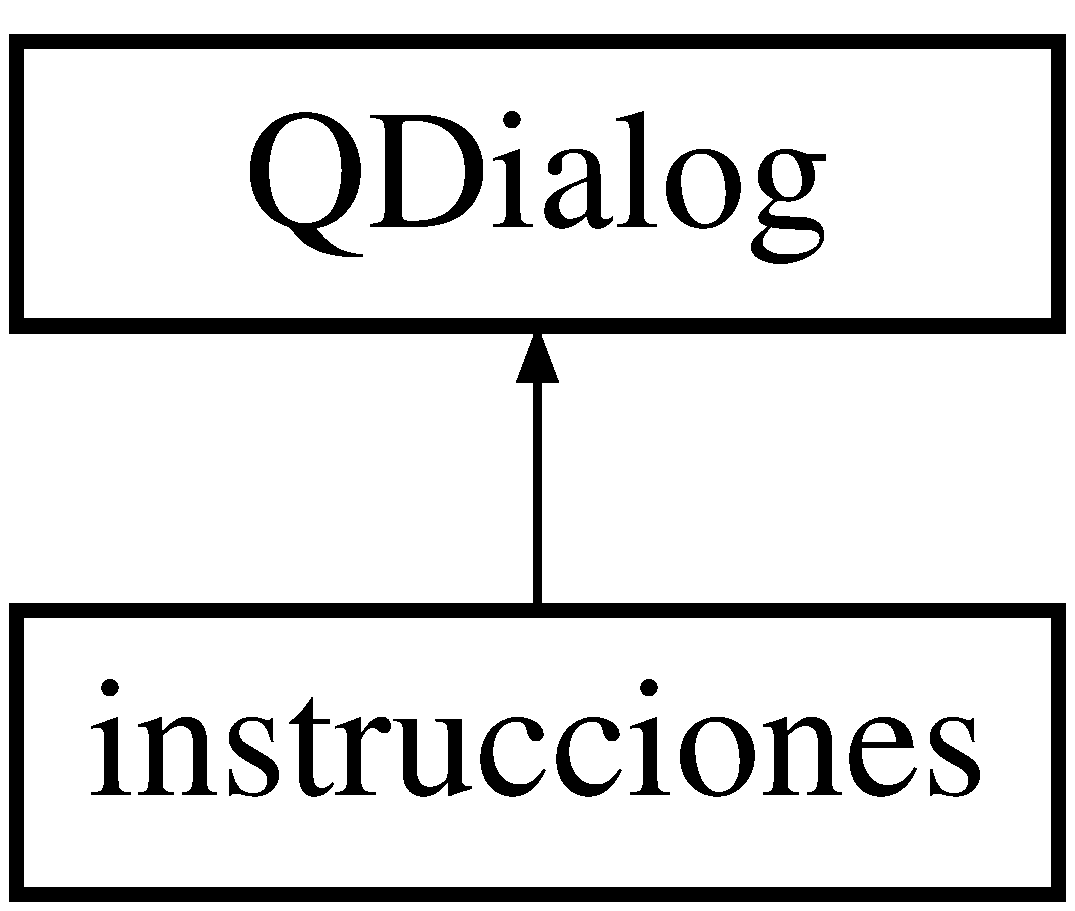
\includegraphics[height=2.000000cm]{classinstrucciones}
\end{center}
\end{figure}
\subsection*{Public Member Functions}
\begin{DoxyCompactItemize}
\item 
\hypertarget{classinstrucciones_a22121db0527da6bbee041cd85c0662dc}{{\bfseries instrucciones} (Q\-Widget $\ast$parent=0)}\label{classinstrucciones_a22121db0527da6bbee041cd85c0662dc}

\end{DoxyCompactItemize}


The documentation for this class was generated from the following files\-:\begin{DoxyCompactItemize}
\item 
\hyperlink{instrucciones_8h}{instrucciones.\-h}\item 
instrucciones.\-cpp\end{DoxyCompactItemize}

\hypertarget{class_jugador}{\section{Jugador Class Reference}
\label{class_jugador}\index{Jugador@{Jugador}}
}
\subsection*{Public Member Functions}
\begin{DoxyCompactItemize}
\item 
\hyperlink{class_jugador_a3921e7cf45f8d7c60ff3c608e64acc7f}{Jugador} (Q\-String n, int p)
\item 
Q\-String \hyperlink{class_jugador_a326995f44b24a9a5247144868f2ba359}{get\-Nombre} ()
\item 
int \hyperlink{class_jugador_a172cd256f90376264170cbab3091a175}{get\-Puntaje} ()
\item 
void \hyperlink{class_jugador_a7409377300d7c5e65b2580944caecef1}{set\-Nombre} (Q\-String n)
\item 
void \hyperlink{class_jugador_ac58c69bef08e23649db0e23f46fd4d44}{set\-Puntaje} (int p)
\end{DoxyCompactItemize}


\subsection{Constructor \& Destructor Documentation}
\hypertarget{class_jugador_a3921e7cf45f8d7c60ff3c608e64acc7f}{\index{Jugador@{Jugador}!Jugador@{Jugador}}
\index{Jugador@{Jugador}!Jugador@{Jugador}}
\subsubsection[{Jugador}]{\setlength{\rightskip}{0pt plus 5cm}Jugador\-::\-Jugador (
\begin{DoxyParamCaption}
\item[{Q\-String}]{n, }
\item[{int}]{p}
\end{DoxyParamCaption}
)}}\label{class_jugador_a3921e7cf45f8d7c60ff3c608e64acc7f}
\hyperlink{class_jugador}{Jugador} constructor de la clase. 
\begin{DoxyParams}{Parameters}
{\em n} & variable de tipo Q\-String que representa el nombre del jugador. \\
\hline
{\em p} & variable de tipo int que representa el puntaje obtenido por el jugador. \\
\hline
\end{DoxyParams}
\begin{DoxyDate}{Date}
07/07/2013 
\end{DoxyDate}


\subsection{Member Function Documentation}
\hypertarget{class_jugador_a326995f44b24a9a5247144868f2ba359}{\index{Jugador@{Jugador}!get\-Nombre@{get\-Nombre}}
\index{get\-Nombre@{get\-Nombre}!Jugador@{Jugador}}
\subsubsection[{get\-Nombre}]{\setlength{\rightskip}{0pt plus 5cm}Q\-String Jugador\-::get\-Nombre (
\begin{DoxyParamCaption}
{}
\end{DoxyParamCaption}
)}}\label{class_jugador_a326995f44b24a9a5247144868f2ba359}
get\-Nombre proporciona el nombre del jugador. \begin{DoxyReturn}{Returns}
una cadena de caracteres con el nombre del jugador. 
\end{DoxyReturn}
\hypertarget{class_jugador_a172cd256f90376264170cbab3091a175}{\index{Jugador@{Jugador}!get\-Puntaje@{get\-Puntaje}}
\index{get\-Puntaje@{get\-Puntaje}!Jugador@{Jugador}}
\subsubsection[{get\-Puntaje}]{\setlength{\rightskip}{0pt plus 5cm}int Jugador\-::get\-Puntaje (
\begin{DoxyParamCaption}
{}
\end{DoxyParamCaption}
)}}\label{class_jugador_a172cd256f90376264170cbab3091a175}
get\-Puntaje proporciona el puntaje obtenido por el jugador. \begin{DoxyReturn}{Returns}
un tipo int con el puntaje almacenado en el jugador. 
\end{DoxyReturn}
\hypertarget{class_jugador_a7409377300d7c5e65b2580944caecef1}{\index{Jugador@{Jugador}!set\-Nombre@{set\-Nombre}}
\index{set\-Nombre@{set\-Nombre}!Jugador@{Jugador}}
\subsubsection[{set\-Nombre}]{\setlength{\rightskip}{0pt plus 5cm}void Jugador\-::set\-Nombre (
\begin{DoxyParamCaption}
\item[{Q\-String}]{n}
\end{DoxyParamCaption}
)}}\label{class_jugador_a7409377300d7c5e65b2580944caecef1}
set\-Nombre cambia el nombre de jugador. 
\begin{DoxyParams}{Parameters}
{\em n} & variable tipo Q\-String que representa el nuevo nombre del jugador. \\
\hline
\end{DoxyParams}
\hypertarget{class_jugador_ac58c69bef08e23649db0e23f46fd4d44}{\index{Jugador@{Jugador}!set\-Puntaje@{set\-Puntaje}}
\index{set\-Puntaje@{set\-Puntaje}!Jugador@{Jugador}}
\subsubsection[{set\-Puntaje}]{\setlength{\rightskip}{0pt plus 5cm}void Jugador\-::set\-Puntaje (
\begin{DoxyParamCaption}
\item[{int}]{p}
\end{DoxyParamCaption}
)}}\label{class_jugador_ac58c69bef08e23649db0e23f46fd4d44}
set\-Puntaje cambia el puntaje de jugador. 
\begin{DoxyParams}{Parameters}
{\em n} & variable tipo int que representa el nuevo puntaje del jugador. \\
\hline
\end{DoxyParams}


The documentation for this class was generated from the following files\-:\begin{DoxyCompactItemize}
\item 
\hyperlink{jugador_8h}{jugador.\-h}\item 
jugador.\-cpp\end{DoxyCompactItemize}

\hypertarget{class_l_c_d_number}{\section{L\-C\-D\-Number Class Reference}
\label{class_l_c_d_number}\index{L\-C\-D\-Number@{L\-C\-D\-Number}}
}
Inheritance diagram for L\-C\-D\-Number\-:\begin{figure}[H]
\begin{center}
\leavevmode
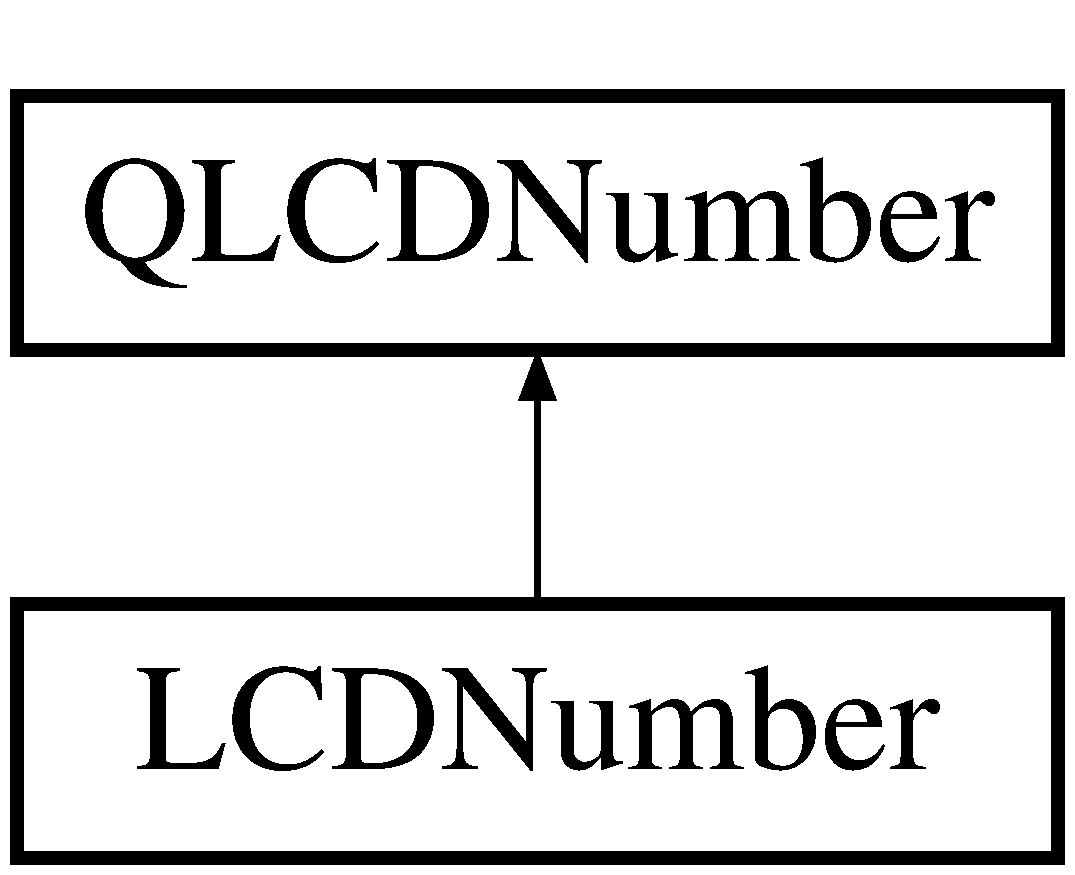
\includegraphics[height=2.000000cm]{class_l_c_d_number}
\end{center}
\end{figure}
\subsection*{Public Slots}
\begin{DoxyCompactItemize}
\item 
\hypertarget{class_l_c_d_number_a7aefd33408d5bde99dac66ec9bf33b19}{void {\bfseries set\-Display} ()}\label{class_l_c_d_number_a7aefd33408d5bde99dac66ec9bf33b19}

\item 
\hypertarget{class_l_c_d_number_a1aab4805806348ba24e3d1c40115b019}{void {\bfseries start} ()}\label{class_l_c_d_number_a1aab4805806348ba24e3d1c40115b019}

\item 
\hypertarget{class_l_c_d_number_ac20c231ee84e02cab47d7b4d73fb86b1}{void {\bfseries stop} ()}\label{class_l_c_d_number_ac20c231ee84e02cab47d7b4d73fb86b1}

\end{DoxyCompactItemize}
\subsection*{Public Member Functions}
\begin{DoxyCompactItemize}
\item 
\hypertarget{class_l_c_d_number_aebf9a2d58b07e6073a8ba260e3395c64}{{\bfseries L\-C\-D\-Number} (int minutes, int seconds)}\label{class_l_c_d_number_aebf9a2d58b07e6073a8ba260e3395c64}

\end{DoxyCompactItemize}
\subsection*{Public Attributes}
\begin{DoxyCompactItemize}
\item 
\hypertarget{class_l_c_d_number_a019f65da6a0b2afb1977f569084d9ca6}{Q\-Timer $\ast$ {\bfseries timer}}\label{class_l_c_d_number_a019f65da6a0b2afb1977f569084d9ca6}

\item 
\hypertarget{class_l_c_d_number_a804920a35b3ec21429797d1aeff89a04}{Q\-Time $\ast$ {\bfseries time\-Value}}\label{class_l_c_d_number_a804920a35b3ec21429797d1aeff89a04}

\end{DoxyCompactItemize}


The documentation for this class was generated from the following files\-:\begin{DoxyCompactItemize}
\item 
\hyperlink{lcdnumber_8h}{lcdnumber.\-h}\item 
lcdnumber.\-cpp\end{DoxyCompactItemize}

\hypertarget{class_ranking}{\section{Ranking Class Reference}
\label{class_ranking}\index{Ranking@{Ranking}}
}
Inheritance diagram for Ranking\-:\begin{figure}[H]
\begin{center}
\leavevmode
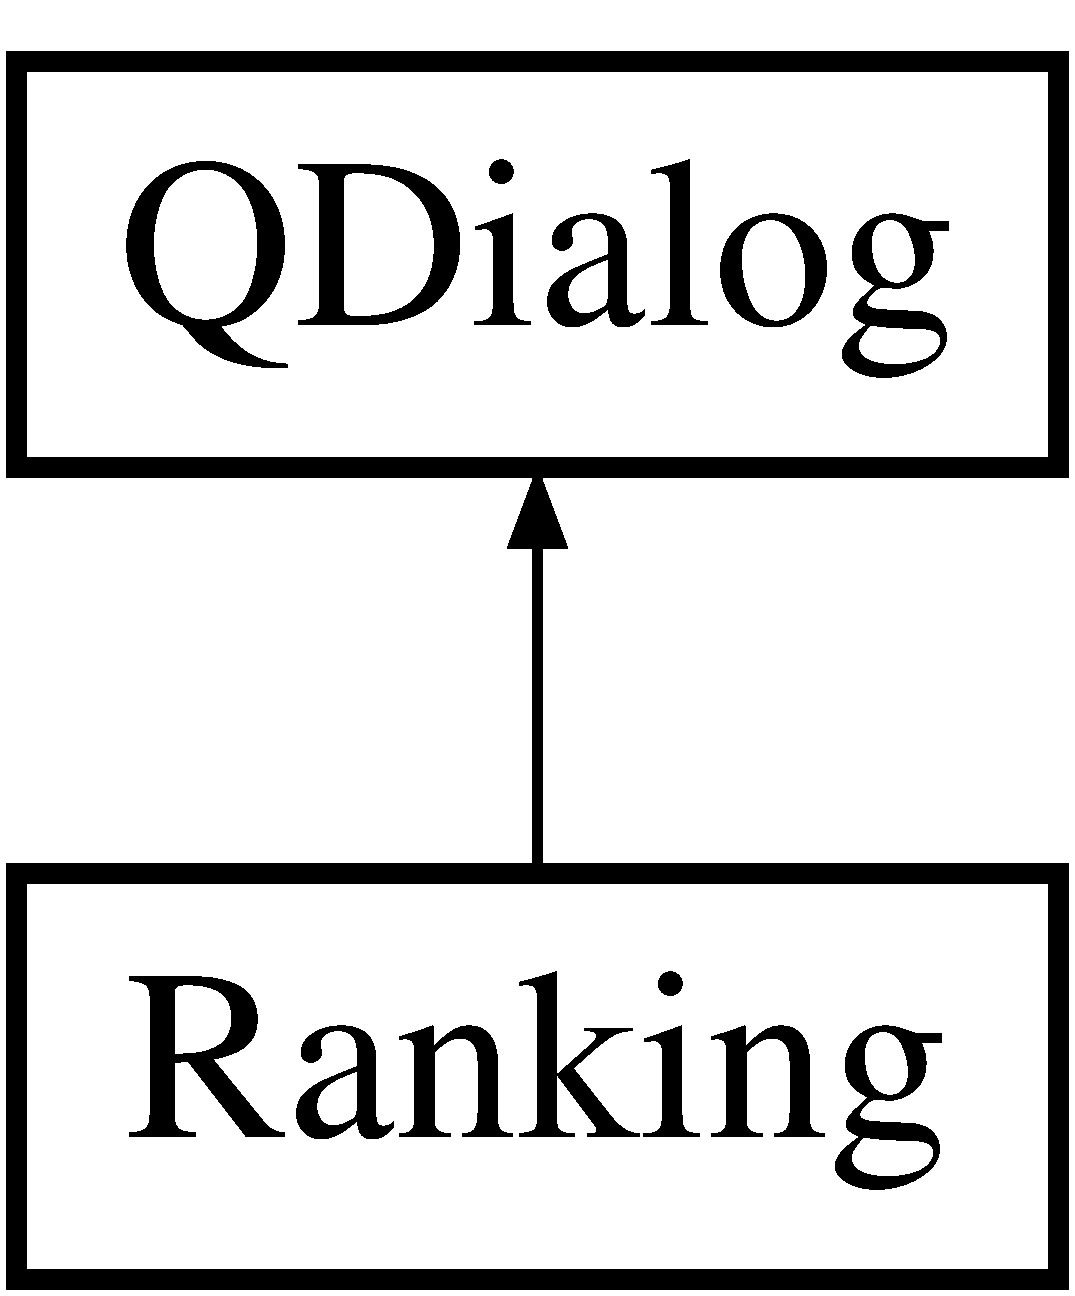
\includegraphics[height=2.000000cm]{class_ranking}
\end{center}
\end{figure}
\subsection*{Public Member Functions}
\begin{DoxyCompactItemize}
\item 
\hypertarget{class_ranking_a01f35fc321e4a359844411a3e4a20ba6}{{\bfseries Ranking} (Q\-Widget $\ast$parent=0)}\label{class_ranking_a01f35fc321e4a359844411a3e4a20ba6}

\item 
Q\-List$<$ \hyperlink{class_jugador}{Jugador} $>$ \hyperlink{class_ranking_a80088e847fbed9d724e03151da18d7b0}{cargar\-Ranking} ()
\item 
Q\-List$<$ \hyperlink{class_jugador}{Jugador} $>$ \hyperlink{class_ranking_a29e0de24fc7bd833d808e707b3979b3e}{ordenar\-Ranking} (Q\-List$<$ \hyperlink{class_jugador}{Jugador} $>$ ranking)
\end{DoxyCompactItemize}


\subsection{Member Function Documentation}
\hypertarget{class_ranking_a80088e847fbed9d724e03151da18d7b0}{\index{Ranking@{Ranking}!cargar\-Ranking@{cargar\-Ranking}}
\index{cargar\-Ranking@{cargar\-Ranking}!Ranking@{Ranking}}
\subsubsection[{cargar\-Ranking}]{\setlength{\rightskip}{0pt plus 5cm}Q\-List$<$ {\bf Jugador} $>$ Ranking\-::cargar\-Ranking (
\begin{DoxyParamCaption}
{}
\end{DoxyParamCaption}
)}}\label{class_ranking_a80088e847fbed9d724e03151da18d7b0}
\hyperlink{class_ranking_a80088e847fbed9d724e03151da18d7b0}{cargar\-Ranking()} permite cargar los elementos que se encuentran almacenado en el archivo de texto ranking.\-txt una vez cargados los elementos se los almacena en un Q\-List$<$\-Jugador$>$ el cual se lo va a retornar. \begin{DoxyReturn}{Returns}
un Q\-List$<$\-Jugador$>$ con los datos de todos los jugadores que han terminado el juego con sus respectivos tiempos. 
\end{DoxyReturn}
\begin{DoxyDate}{Date}
07/07/2013 
\end{DoxyDate}
\hypertarget{class_ranking_a29e0de24fc7bd833d808e707b3979b3e}{\index{Ranking@{Ranking}!ordenar\-Ranking@{ordenar\-Ranking}}
\index{ordenar\-Ranking@{ordenar\-Ranking}!Ranking@{Ranking}}
\subsubsection[{ordenar\-Ranking}]{\setlength{\rightskip}{0pt plus 5cm}Q\-List$<$ {\bf Jugador} $>$ Ranking\-::ordenar\-Ranking (
\begin{DoxyParamCaption}
\item[{Q\-List$<$ {\bf Jugador} $>$}]{ranking}
\end{DoxyParamCaption}
)}}\label{class_ranking_a29e0de24fc7bd833d808e707b3979b3e}
\hyperlink{class_ranking_a29e0de24fc7bd833d808e707b3979b3e}{ordenar\-Ranking()} permite ordenar de los elementos de la lista de manera ascedente tomando como referencia de comparación el tiempo que se tomo en finalizar el juego. 
\begin{DoxyParams}{Parameters}
{\em una} & variable de tipo Q\-List$<$\-Jugador$>$ donde se encuentran los jugadores obtenidos del archivo ranking.\-txt. \\
\hline
\end{DoxyParams}
\begin{DoxyReturn}{Returns}
un Q\-List$<$\-Jugador$>$ con los datos ordenado de manera ascendente. 
\end{DoxyReturn}
\begin{DoxyDate}{Date}
07/07/2013 
\end{DoxyDate}


The documentation for this class was generated from the following files\-:\begin{DoxyCompactItemize}
\item 
\hyperlink{ranking_8h}{ranking.\-h}\item 
ranking.\-cpp\end{DoxyCompactItemize}

\hypertarget{classsudoku}{\section{sudoku Class Reference}
\label{classsudoku}\index{sudoku@{sudoku}}
}
Inheritance diagram for sudoku\-:\begin{figure}[H]
\begin{center}
\leavevmode
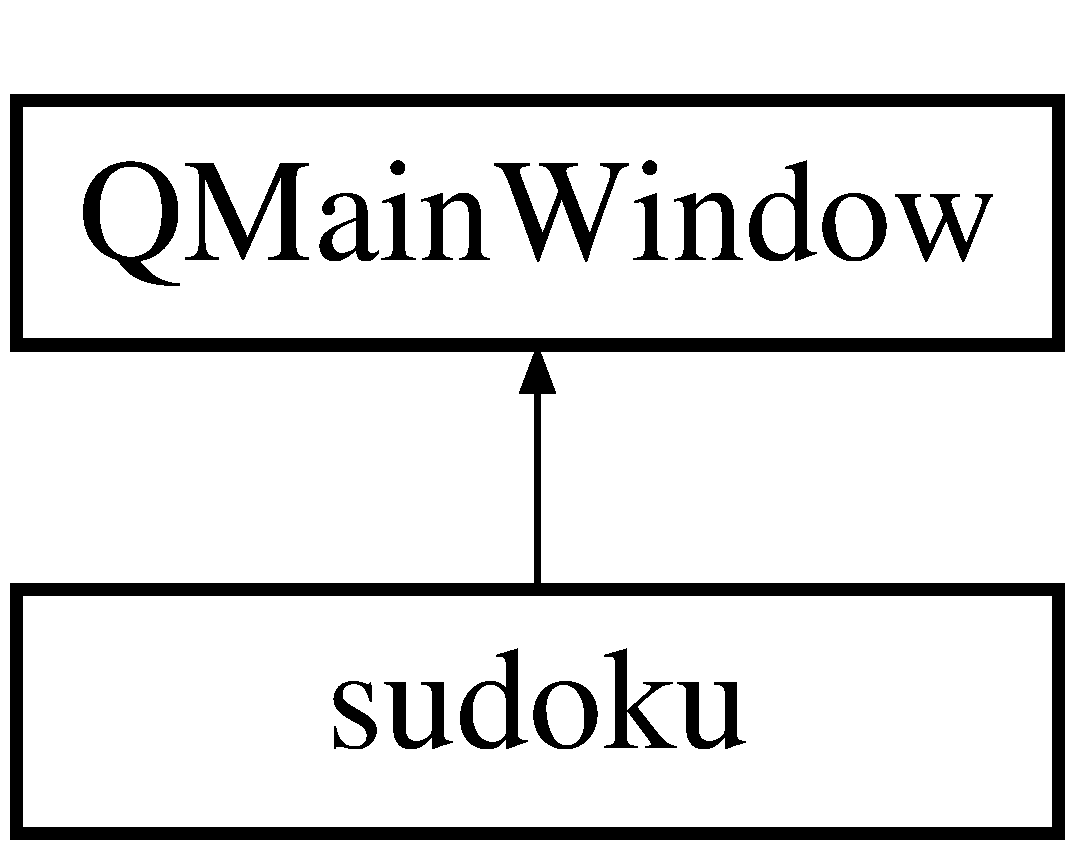
\includegraphics[height=2.000000cm]{classsudoku}
\end{center}
\end{figure}
\subsection*{Public Member Functions}
\begin{DoxyCompactItemize}
\item 
\hypertarget{classsudoku_a4fca394ee6b069056fa9e12ad5636e2a}{{\bfseries sudoku} (Q\-Widget $\ast$parent=0, int dificultad=0, Q\-String nom\-Jugador=\char`\"{}\char`\"{})}\label{classsudoku_a4fca394ee6b069056fa9e12ad5636e2a}

\item 
void \hyperlink{classsudoku_a617ded672f64a712fdb32cdb39587e41}{llenarsudoku} (int dif, Q\-String nom)
\item 
int \hyperlink{classsudoku_a9eb0e3df6cdeda0dd3895e982c8eb639}{verificar\-Horizontal} (int matriz\mbox{[}9\mbox{]}\mbox{[}9\mbox{]}, int x, int y)
\item 
int \hyperlink{classsudoku_aae809634b98c50419673cbfbeeed1424}{verificar\-Vertical} (int matriz\mbox{[}9\mbox{]}\mbox{[}9\mbox{]}, int x, int y)
\item 
int \hyperlink{classsudoku_a1b70089b6aa10d82a1221cd393e317d4}{verificar\-Recuadro} (int matriz\mbox{[}9\mbox{]}\mbox{[}9\mbox{]}, int x, int y)
\item 
int \hyperlink{classsudoku_a666728002336616bf9c8443574e2a0a2}{verificar\-Sudoku} (int matriz\mbox{[}9\mbox{]}\mbox{[}9\mbox{]})
\item 
void \hyperlink{classsudoku_a050dfc7ca3f27165923db48d7b3fafd9}{sacar\-Ceros} ()
\item 
void \hyperlink{classsudoku_a0a1d90110883ce8af57b1b3aeef28567}{llenar\-Ceros} (int matriz\mbox{[}9\mbox{]}\mbox{[}9\mbox{]})
\item 
int \hyperlink{classsudoku_ab7095d78fa0050d8b4f33ae71afd7ddd}{es\-Posible} (int posibilidad, int matriz\mbox{[}9\mbox{]}\mbox{[}9\mbox{]}, int pos\-X, int pos\-Y)
\item 
Q\-List$<$ int $>$ \hyperlink{classsudoku_af1d2b7818b60dac0845d719f0aec9cb2}{reiniciar} (int matriz\mbox{[}9\mbox{]}\mbox{[}9\mbox{]}, int pos\-X, int pos\-Y)
\item 
Q\-List$<$ int $>$ \hyperlink{classsudoku_a781664045c5796e65aaeef1e7f7f26d5}{lista\-De\-Posibilidades} (int matriz\mbox{[}9\mbox{]}\mbox{[}9\mbox{]}, int pos\-X, int pos\-Y)
\item 
void \hyperlink{classsudoku_ac3f30cbd81fbb88c7da0e4aaa9fc2e7a}{copiar\-Matriz} (int matriz\mbox{[}9\mbox{]}\mbox{[}9\mbox{]}, int matriz\-Copia\mbox{[}9\mbox{]}\mbox{[}9\mbox{]})
\item 
void \hyperlink{classsudoku_a523bdf77cfc3221b46a2ef2ef6f35dc7}{colocar\-Pistas} (int matriz\mbox{[}9\mbox{]}\mbox{[}9\mbox{]}, int matriz\-Sudoku\mbox{[}9\mbox{]}\mbox{[}9\mbox{]}, int num\-Pistas)
\item 
void \hyperlink{classsudoku_a382e974f9b268bad72349e835046bc9e}{guardar\-Partida} ()
\item 
void \hyperlink{classsudoku_ab810a66d51bbe7abef401fff3bbeab66}{obtener\-Matriz} (int matriz\mbox{[}9\mbox{]}\mbox{[}9\mbox{]})
\item 
void \hyperlink{classsudoku_a609094f632cbb607bcf4ccc6c5163ee6}{pista\-Jugador} ()
\item 
void \hyperlink{classsudoku_a557f08c7f68d6f464cf55b6cb263e4f1}{jugadas\-Incorrectas} ()
\item 
void \hyperlink{classsudoku_aa59a6bcde7a2de2b8522ca45de7e7fda}{jugadas\-Invalidas} ()
\item 
Q\-String \hyperlink{classsudoku_a801aaa352372d14d0e782c74e59dcffd}{encriptar} (int num)
\item 
int \hyperlink{classsudoku_a38e9561028b7e53bcb33a7b41301a25c}{decode} (Q\-String code)
\item 
void \hyperlink{classsudoku_a52516f05ede755c0a383d0ead1eb7f98}{cargar\-Partida} ()
\item 
void \hyperlink{classsudoku_aaf120f44b1fb018460832c90f3411115}{cargar\-Solucion} ()
\item 
void \hyperlink{classsudoku_a56f04c8bd9362116a7d558a58a621167}{guardar\-Solucion} ()
\item 
void \hyperlink{classsudoku_a422ab0aa3c2044ee421283a69270ac38}{cargar\-Original} ()
\item 
void \hyperlink{classsudoku_a7bd027391311e65fc690df2f3bc67a44}{guardar\-Original} ()
\item 
Q\-List$<$ \hyperlink{class_jugador}{Jugador} $>$ \hyperlink{classsudoku_aed2f8fec3117c5a7cb8c3a2f510a28c9}{cargar\-Ranking} ()
\begin{DoxyCompactList}\small\item\em cargar\-Ranking obtiene los datos almacenado en el archivo \char`\"{}ranking.\-txt\char`\"{}. \end{DoxyCompactList}\item 
void \hyperlink{classsudoku_a2811b7d6ec908b16314a6ff6ec2659dc}{guardar\-Ranking} (int puntaje)
\begin{DoxyCompactList}\small\item\em guardar\-Ranking guarda el elemento una vez concluida la partida de forma exitosa. \end{DoxyCompactList}\end{DoxyCompactItemize}
\subsection*{Public Attributes}
\begin{DoxyCompactItemize}
\item 
\hypertarget{classsudoku_afde53a179f11c54b772a8723929b3a7b}{Q\-List$<$ int $>$ {\bfseries list\-Pos\-X}}\label{classsudoku_afde53a179f11c54b772a8723929b3a7b}

\item 
\hypertarget{classsudoku_a26df7ff7d6715034015c965ddb8c9c5e}{Q\-List$<$ int $>$ {\bfseries list\-Pos\-Y}}\label{classsudoku_a26df7ff7d6715034015c965ddb8c9c5e}

\item 
\hypertarget{classsudoku_ae0cee3e3b8b57d8ac65a9d0f88201ea6}{int {\bfseries matriz} \mbox{[}9\mbox{]}\mbox{[}9\mbox{]}}\label{classsudoku_ae0cee3e3b8b57d8ac65a9d0f88201ea6}

\item 
\hypertarget{classsudoku_a75b7e268f5cd8124fa4455081a5a2941}{int {\bfseries matriz\-Sudoku} \mbox{[}9\mbox{]}\mbox{[}9\mbox{]}}\label{classsudoku_a75b7e268f5cd8124fa4455081a5a2941}

\end{DoxyCompactItemize}


\subsection{Member Function Documentation}
\hypertarget{classsudoku_a422ab0aa3c2044ee421283a69270ac38}{\index{sudoku@{sudoku}!cargar\-Original@{cargar\-Original}}
\index{cargar\-Original@{cargar\-Original}!sudoku@{sudoku}}
\subsubsection[{cargar\-Original}]{\setlength{\rightskip}{0pt plus 5cm}void sudoku\-::cargar\-Original (
\begin{DoxyParamCaption}
{}
\end{DoxyParamCaption}
)}}\label{classsudoku_a422ab0aa3c2044ee421283a69270ac38}
cargar\-Original carga los datos almacenado en el archivo \char`\"{}guardar\-O.\-txt\char`\"{}. \begin{DoxyDate}{Date}
07/07/2013 
\end{DoxyDate}
\hypertarget{classsudoku_a52516f05ede755c0a383d0ead1eb7f98}{\index{sudoku@{sudoku}!cargar\-Partida@{cargar\-Partida}}
\index{cargar\-Partida@{cargar\-Partida}!sudoku@{sudoku}}
\subsubsection[{cargar\-Partida}]{\setlength{\rightskip}{0pt plus 5cm}void sudoku\-::cargar\-Partida (
\begin{DoxyParamCaption}
{}
\end{DoxyParamCaption}
)}}\label{classsudoku_a52516f05ede755c0a383d0ead1eb7f98}
cargar\-Partida carga los datos almacenado en el archivo \char`\"{}guardar.\-txt\char`\"{}. \begin{DoxyDate}{Date}
07/07/2013 
\end{DoxyDate}
\hypertarget{classsudoku_aed2f8fec3117c5a7cb8c3a2f510a28c9}{\index{sudoku@{sudoku}!cargar\-Ranking@{cargar\-Ranking}}
\index{cargar\-Ranking@{cargar\-Ranking}!sudoku@{sudoku}}
\subsubsection[{cargar\-Ranking}]{\setlength{\rightskip}{0pt plus 5cm}Q\-List$<$ {\bf Jugador} $>$ sudoku\-::cargar\-Ranking (
\begin{DoxyParamCaption}
{}
\end{DoxyParamCaption}
)}}\label{classsudoku_aed2f8fec3117c5a7cb8c3a2f510a28c9}


cargar\-Ranking obtiene los datos almacenado en el archivo \char`\"{}ranking.\-txt\char`\"{}. 

\begin{DoxyReturn}{Returns}
Q\-List$<$\-Jugador$>$ una lista con los jugadores que se encuentran en el archivo de texto. 
\end{DoxyReturn}
\hypertarget{classsudoku_aaf120f44b1fb018460832c90f3411115}{\index{sudoku@{sudoku}!cargar\-Solucion@{cargar\-Solucion}}
\index{cargar\-Solucion@{cargar\-Solucion}!sudoku@{sudoku}}
\subsubsection[{cargar\-Solucion}]{\setlength{\rightskip}{0pt plus 5cm}void sudoku\-::cargar\-Solucion (
\begin{DoxyParamCaption}
{}
\end{DoxyParamCaption}
)}}\label{classsudoku_aaf120f44b1fb018460832c90f3411115}
cargar\-Solucion carga los datos almacenado en el archivo \char`\"{}guardar\-S.\-txt\char`\"{}. \begin{DoxyDate}{Date}
07/07/2013 
\end{DoxyDate}
\hypertarget{classsudoku_a523bdf77cfc3221b46a2ef2ef6f35dc7}{\index{sudoku@{sudoku}!colocar\-Pistas@{colocar\-Pistas}}
\index{colocar\-Pistas@{colocar\-Pistas}!sudoku@{sudoku}}
\subsubsection[{colocar\-Pistas}]{\setlength{\rightskip}{0pt plus 5cm}void sudoku\-::colocar\-Pistas (
\begin{DoxyParamCaption}
\item[{int}]{matriz\mbox{[}9\mbox{]}\mbox{[}9\mbox{]}, }
\item[{int}]{matriz\-Sudoku\mbox{[}9\mbox{]}\mbox{[}9\mbox{]}, }
\item[{int}]{num\-Pistas}
\end{DoxyParamCaption}
)}}\label{classsudoku_a523bdf77cfc3221b46a2ef2ef6f35dc7}
colocar\-Pistas se colocan pista para que se pueda resolver el sudoku de acuerdo al nivel seleccionado. 
\begin{DoxyParams}{Parameters}
{\em matriz} & variable int 9x9 matriz que contiene el sudoku resuelto. \\
\hline
{\em matriz\-Sudoku} & variable int 9x9 matriz la cual se le va a colocar las pista y posteriormente se la presenta en la interfaz grafica. \\
\hline
{\em num\-Pistas} & variable tipo int la cual nos proporciona cuantas pista se le da al jugador. \\
\hline
\end{DoxyParams}
\begin{DoxyDate}{Date}
07/07/2013 
\end{DoxyDate}
\hypertarget{classsudoku_ac3f30cbd81fbb88c7da0e4aaa9fc2e7a}{\index{sudoku@{sudoku}!copiar\-Matriz@{copiar\-Matriz}}
\index{copiar\-Matriz@{copiar\-Matriz}!sudoku@{sudoku}}
\subsubsection[{copiar\-Matriz}]{\setlength{\rightskip}{0pt plus 5cm}void sudoku\-::copiar\-Matriz (
\begin{DoxyParamCaption}
\item[{int}]{matriz\mbox{[}9\mbox{]}\mbox{[}9\mbox{]}, }
\item[{int}]{matriz\-Copia\mbox{[}9\mbox{]}\mbox{[}9\mbox{]}}
\end{DoxyParamCaption}
)}}\label{classsudoku_ac3f30cbd81fbb88c7da0e4aaa9fc2e7a}
copiar\-Matriz hace una copia de la matriz. 
\begin{DoxyParams}{Parameters}
{\em matriz} & variable int 9x9 matriz la cual se va a sacar una copia. \\
\hline
{\em matriz\-Copia} & variable int 9x9 en la cual se va a llenar con los elementos que se encuentran en la variable matriz. \\
\hline
\end{DoxyParams}
\begin{DoxyDate}{Date}
07/07/2013 
\end{DoxyDate}
\hypertarget{classsudoku_a38e9561028b7e53bcb33a7b41301a25c}{\index{sudoku@{sudoku}!decode@{decode}}
\index{decode@{decode}!sudoku@{sudoku}}
\subsubsection[{decode}]{\setlength{\rightskip}{0pt plus 5cm}int sudoku\-::decode (
\begin{DoxyParamCaption}
\item[{Q\-String}]{code}
\end{DoxyParamCaption}
)}}\label{classsudoku_a38e9561028b7e53bcb33a7b41301a25c}
decode decodifica la cadena de caracteres que se envia por parametro. 
\begin{DoxyParams}{Parameters}
{\em code} & variable tipo Q\-String el cual va a ser decodificado. \\
\hline
\end{DoxyParams}
\begin{DoxyReturn}{Returns}
int que representa la decodificado de la cadena de caracteres . 
\end{DoxyReturn}
\begin{DoxyDate}{Date}
07/07/2013 
\end{DoxyDate}
\hypertarget{classsudoku_a801aaa352372d14d0e782c74e59dcffd}{\index{sudoku@{sudoku}!encriptar@{encriptar}}
\index{encriptar@{encriptar}!sudoku@{sudoku}}
\subsubsection[{encriptar}]{\setlength{\rightskip}{0pt plus 5cm}Q\-String sudoku\-::encriptar (
\begin{DoxyParamCaption}
\item[{int}]{num}
\end{DoxyParamCaption}
)}}\label{classsudoku_a801aaa352372d14d0e782c74e59dcffd}
encriptar codifica el numero envia por parametro. 
\begin{DoxyParams}{Parameters}
{\em num} & variable tipo int el cual va a ser codificado. \\
\hline
\end{DoxyParams}
\begin{DoxyReturn}{Returns}
Q\-String que representa una cadena de caracteres del numero codificado. 
\end{DoxyReturn}
\begin{DoxyDate}{Date}
07/07/2013 
\end{DoxyDate}
\hypertarget{classsudoku_ab7095d78fa0050d8b4f33ae71afd7ddd}{\index{sudoku@{sudoku}!es\-Posible@{es\-Posible}}
\index{es\-Posible@{es\-Posible}!sudoku@{sudoku}}
\subsubsection[{es\-Posible}]{\setlength{\rightskip}{0pt plus 5cm}int sudoku\-::es\-Posible (
\begin{DoxyParamCaption}
\item[{int}]{posibilidad, }
\item[{int}]{matriz\mbox{[}9\mbox{]}\mbox{[}9\mbox{]}, }
\item[{int}]{pos\-X, }
\item[{int}]{pos\-Y}
\end{DoxyParamCaption}
)}}\label{classsudoku_ab7095d78fa0050d8b4f33ae71afd7ddd}
es\-Posible hace una verificacion si el numero deseado es una opcion valida a colocar en la casilla actual. 
\begin{DoxyParams}{Parameters}
{\em posibilidad} & variable tipo int que representa el numero que se va a colocar en la casilla. \\
\hline
{\em matriz} & variable int 9x9 que representa al sudoku \\
\hline
{\em x} & variable int que representa la posicion x de la casilla que se quiere verificar. \\
\hline
{\em y} & variable int que representa la posicion y de la casilla que se quiere verificar. \\
\hline
\end{DoxyParams}
\begin{DoxyReturn}{Returns}
un tipo int que retorna 0 cuando el numero proporcionado es valido y 1 cuando es invalido. 
\end{DoxyReturn}
\begin{DoxyDate}{Date}
07/07/2013 
\end{DoxyDate}
\hypertarget{classsudoku_a7bd027391311e65fc690df2f3bc67a44}{\index{sudoku@{sudoku}!guardar\-Original@{guardar\-Original}}
\index{guardar\-Original@{guardar\-Original}!sudoku@{sudoku}}
\subsubsection[{guardar\-Original}]{\setlength{\rightskip}{0pt plus 5cm}void sudoku\-::guardar\-Original (
\begin{DoxyParamCaption}
{}
\end{DoxyParamCaption}
)}}\label{classsudoku_a7bd027391311e65fc690df2f3bc67a44}
guardar\-Original crea un archivo txt con los datos iniciales de la partida actual. \begin{DoxyDate}{Date}
07/07/2013 
\end{DoxyDate}
\hypertarget{classsudoku_a382e974f9b268bad72349e835046bc9e}{\index{sudoku@{sudoku}!guardar\-Partida@{guardar\-Partida}}
\index{guardar\-Partida@{guardar\-Partida}!sudoku@{sudoku}}
\subsubsection[{guardar\-Partida}]{\setlength{\rightskip}{0pt plus 5cm}void sudoku\-::guardar\-Partida (
\begin{DoxyParamCaption}
{}
\end{DoxyParamCaption}
)}}\label{classsudoku_a382e974f9b268bad72349e835046bc9e}
guardar\-Partida crea un archivo txt con los datos de la partida actual. \begin{DoxyDate}{Date}
07/07/2013 
\end{DoxyDate}
\hypertarget{classsudoku_a2811b7d6ec908b16314a6ff6ec2659dc}{\index{sudoku@{sudoku}!guardar\-Ranking@{guardar\-Ranking}}
\index{guardar\-Ranking@{guardar\-Ranking}!sudoku@{sudoku}}
\subsubsection[{guardar\-Ranking}]{\setlength{\rightskip}{0pt plus 5cm}void sudoku\-::guardar\-Ranking (
\begin{DoxyParamCaption}
\item[{int}]{puntaje}
\end{DoxyParamCaption}
)}}\label{classsudoku_a2811b7d6ec908b16314a6ff6ec2659dc}


guardar\-Ranking guarda el elemento una vez concluida la partida de forma exitosa. 


\begin{DoxyParams}{Parameters}
{\em puntaje} & se guarda en el archivo el nuevo elemento. \\
\hline
\end{DoxyParams}
\hypertarget{classsudoku_a56f04c8bd9362116a7d558a58a621167}{\index{sudoku@{sudoku}!guardar\-Solucion@{guardar\-Solucion}}
\index{guardar\-Solucion@{guardar\-Solucion}!sudoku@{sudoku}}
\subsubsection[{guardar\-Solucion}]{\setlength{\rightskip}{0pt plus 5cm}void sudoku\-::guardar\-Solucion (
\begin{DoxyParamCaption}
{}
\end{DoxyParamCaption}
)}}\label{classsudoku_a56f04c8bd9362116a7d558a58a621167}
guardar\-Solucion crea un archivo txt con los datos del sudoku resuelto de la partida actual. \begin{DoxyDate}{Date}
07/07/2013 
\end{DoxyDate}
\hypertarget{classsudoku_a557f08c7f68d6f464cf55b6cb263e4f1}{\index{sudoku@{sudoku}!jugadas\-Incorrectas@{jugadas\-Incorrectas}}
\index{jugadas\-Incorrectas@{jugadas\-Incorrectas}!sudoku@{sudoku}}
\subsubsection[{jugadas\-Incorrectas}]{\setlength{\rightskip}{0pt plus 5cm}void sudoku\-::jugadas\-Incorrectas (
\begin{DoxyParamCaption}
{}
\end{DoxyParamCaption}
)}}\label{classsudoku_a557f08c7f68d6f464cf55b6cb263e4f1}
jugadas\-Incorrectas se verifica en funcion al tablero resuelto. \begin{DoxyDate}{Date}
07/07/2013 
\end{DoxyDate}
\hypertarget{classsudoku_aa59a6bcde7a2de2b8522ca45de7e7fda}{\index{sudoku@{sudoku}!jugadas\-Invalidas@{jugadas\-Invalidas}}
\index{jugadas\-Invalidas@{jugadas\-Invalidas}!sudoku@{sudoku}}
\subsubsection[{jugadas\-Invalidas}]{\setlength{\rightskip}{0pt plus 5cm}void sudoku\-::jugadas\-Invalidas (
\begin{DoxyParamCaption}
{}
\end{DoxyParamCaption}
)}}\label{classsudoku_aa59a6bcde7a2de2b8522ca45de7e7fda}
jugadas\-Invalidas no validas segun el estado actual del tablero. \begin{DoxyDate}{Date}
07/07/2013 
\end{DoxyDate}
\hypertarget{classsudoku_a781664045c5796e65aaeef1e7f7f26d5}{\index{sudoku@{sudoku}!lista\-De\-Posibilidades@{lista\-De\-Posibilidades}}
\index{lista\-De\-Posibilidades@{lista\-De\-Posibilidades}!sudoku@{sudoku}}
\subsubsection[{lista\-De\-Posibilidades}]{\setlength{\rightskip}{0pt plus 5cm}Q\-List$<$ int $>$ sudoku\-::lista\-De\-Posibilidades (
\begin{DoxyParamCaption}
\item[{int}]{matriz\mbox{[}9\mbox{]}\mbox{[}9\mbox{]}, }
\item[{int}]{pos\-X, }
\item[{int}]{pos\-Y}
\end{DoxyParamCaption}
)}}\label{classsudoku_a781664045c5796e65aaeef1e7f7f26d5}
lista\-De\-Posibilidades creo una lista con todos lo numero posibles que se pueden colocar en la casilla seleccionada. 
\begin{DoxyParams}{Parameters}
{\em matriz} & variable int 9x9 que representa al sudoku \\
\hline
{\em x} & variable int que representa la posicion x de la casilla que se quiere verificar. \\
\hline
{\em y} & variable int que representa la posicion y de la casilla que se quiere verificar. \\
\hline
\end{DoxyParams}
\begin{DoxyReturn}{Returns}
un tipo int que retorna 0 cuando el numero proporcionado es valido y 1 cuando es invalido. 
\end{DoxyReturn}
\begin{DoxyDate}{Date}
07/07/2013 
\end{DoxyDate}
\hypertarget{classsudoku_a0a1d90110883ce8af57b1b3aeef28567}{\index{sudoku@{sudoku}!llenar\-Ceros@{llenar\-Ceros}}
\index{llenar\-Ceros@{llenar\-Ceros}!sudoku@{sudoku}}
\subsubsection[{llenar\-Ceros}]{\setlength{\rightskip}{0pt plus 5cm}void sudoku\-::llenar\-Ceros (
\begin{DoxyParamCaption}
\item[{int}]{matriz\mbox{[}9\mbox{]}\mbox{[}9\mbox{]}}
\end{DoxyParamCaption}
)}}\label{classsudoku_a0a1d90110883ce8af57b1b3aeef28567}
llenar\-Ceros llena toda la matriz con 0. 
\begin{DoxyParams}{Parameters}
{\em matriz} & variable int 9x9. \\
\hline
\end{DoxyParams}
\begin{DoxyDate}{Date}
07/07/2013 
\end{DoxyDate}
\hypertarget{classsudoku_a617ded672f64a712fdb32cdb39587e41}{\index{sudoku@{sudoku}!llenarsudoku@{llenarsudoku}}
\index{llenarsudoku@{llenarsudoku}!sudoku@{sudoku}}
\subsubsection[{llenarsudoku}]{\setlength{\rightskip}{0pt plus 5cm}void sudoku\-::llenarsudoku (
\begin{DoxyParamCaption}
\item[{int}]{dif, }
\item[{Q\-String}]{nom}
\end{DoxyParamCaption}
)}}\label{classsudoku_a617ded672f64a712fdb32cdb39587e41}
llenarsudoku se encarga de la creacion y presentacion en la ventana de juego del sudoku 
\begin{DoxyParams}{Parameters}
{\em dif} & \\
\hline
{\em nom} & variable Q\-String que representa el nombre del jugador actual. \\
\hline
\end{DoxyParams}
\begin{DoxyDate}{Date}
07/07/2013 
\end{DoxyDate}
\hypertarget{classsudoku_ab810a66d51bbe7abef401fff3bbeab66}{\index{sudoku@{sudoku}!obtener\-Matriz@{obtener\-Matriz}}
\index{obtener\-Matriz@{obtener\-Matriz}!sudoku@{sudoku}}
\subsubsection[{obtener\-Matriz}]{\setlength{\rightskip}{0pt plus 5cm}void sudoku\-::obtener\-Matriz (
\begin{DoxyParamCaption}
\item[{int}]{matriz\mbox{[}9\mbox{]}\mbox{[}9\mbox{]}}
\end{DoxyParamCaption}
)}}\label{classsudoku_ab810a66d51bbe7abef401fff3bbeab66}
obtener\-Matriz obtiene los datos del sudoku que se encuentran en la interfaz grafica. 
\begin{DoxyParams}{Parameters}
{\em matriz} & variable int 9x9 matriz se le añaden los elementos que son proporcionado por la interfaz. \\
\hline
\end{DoxyParams}
\begin{DoxyDate}{Date}
07/07/2013 
\end{DoxyDate}
\hypertarget{classsudoku_a609094f632cbb607bcf4ccc6c5163ee6}{\index{sudoku@{sudoku}!pista\-Jugador@{pista\-Jugador}}
\index{pista\-Jugador@{pista\-Jugador}!sudoku@{sudoku}}
\subsubsection[{pista\-Jugador}]{\setlength{\rightskip}{0pt plus 5cm}void sudoku\-::pista\-Jugador (
\begin{DoxyParamCaption}
{}
\end{DoxyParamCaption}
)}}\label{classsudoku_a609094f632cbb607bcf4ccc6c5163ee6}
pista\-Jugador coloca un numero que todavia no a sido puesto en el tablero. \begin{DoxyDate}{Date}
07/07/2013 
\end{DoxyDate}
\hypertarget{classsudoku_af1d2b7818b60dac0845d719f0aec9cb2}{\index{sudoku@{sudoku}!reiniciar@{reiniciar}}
\index{reiniciar@{reiniciar}!sudoku@{sudoku}}
\subsubsection[{reiniciar}]{\setlength{\rightskip}{0pt plus 5cm}Q\-List$<$ int $>$ sudoku\-::reiniciar (
\begin{DoxyParamCaption}
\item[{int}]{matriz\mbox{[}9\mbox{]}\mbox{[}9\mbox{]}, }
\item[{int}]{pos\-X, }
\item[{int}]{pos\-Y}
\end{DoxyParamCaption}
)}}\label{classsudoku_af1d2b7818b60dac0845d719f0aec9cb2}
reiniciar elimina todo los elemento ingresados distintos de 0 que se encuentra en la fila, columna y recuadro del sudoku. 
\begin{DoxyParams}{Parameters}
{\em matriz} & variable int 9x9 que representa al sudoku \\
\hline
{\em x} & variable int que representa la posicion x de la casilla que se quiere verificar. \\
\hline
{\em y} & variable int que representa la posicion y de la casilla que se quiere verificar. \\
\hline
\end{DoxyParams}
\begin{DoxyReturn}{Returns}
un Q\-List$<$int$>$ con todas la posiciones de los elementos removidos donde se han ingresado un elemento distinto de 0. 
\end{DoxyReturn}
\begin{DoxyDate}{Date}
07/07/2013 
\end{DoxyDate}
\hypertarget{classsudoku_a050dfc7ca3f27165923db48d7b3fafd9}{\index{sudoku@{sudoku}!sacar\-Ceros@{sacar\-Ceros}}
\index{sacar\-Ceros@{sacar\-Ceros}!sudoku@{sudoku}}
\subsubsection[{sacar\-Ceros}]{\setlength{\rightskip}{0pt plus 5cm}void sudoku\-::sacar\-Ceros (
\begin{DoxyParamCaption}
{}
\end{DoxyParamCaption}
)}}\label{classsudoku_a050dfc7ca3f27165923db48d7b3fafd9}
sacar\-Ceros remueve los ceros que se han añadido a las interfaz grafica y los reemplazo por \char`\"{}\char`\"{}. \begin{DoxyDate}{Date}
07/07/2013 
\end{DoxyDate}
\hypertarget{classsudoku_a9eb0e3df6cdeda0dd3895e982c8eb639}{\index{sudoku@{sudoku}!verificar\-Horizontal@{verificar\-Horizontal}}
\index{verificar\-Horizontal@{verificar\-Horizontal}!sudoku@{sudoku}}
\subsubsection[{verificar\-Horizontal}]{\setlength{\rightskip}{0pt plus 5cm}int sudoku\-::verificar\-Horizontal (
\begin{DoxyParamCaption}
\item[{int}]{matriz\mbox{[}9\mbox{]}\mbox{[}9\mbox{]}, }
\item[{int}]{x, }
\item[{int}]{y}
\end{DoxyParamCaption}
)}}\label{classsudoku_a9eb0e3df6cdeda0dd3895e982c8eb639}
verificar\-Horizontal permite hacer la validacion de toda la fila si es que cumple las reglas del sudoku. 
\begin{DoxyParams}{Parameters}
{\em matriz} & variable int 9x9 que representa al sudoku \\
\hline
{\em x} & variable int que representa la posicion x de la casilla que se quiere verificar. \\
\hline
{\em y} & variable int que representa la posicion y de la casilla que se quiere verificar. \\
\hline
\end{DoxyParams}
\begin{DoxyReturn}{Returns}
un tipo int que retorna 0 cuando la casilla verificada es correcta y 1 cuando es incorrecta. 
\end{DoxyReturn}
\begin{DoxyDate}{Date}
07/07/2013 
\end{DoxyDate}
\hypertarget{classsudoku_a1b70089b6aa10d82a1221cd393e317d4}{\index{sudoku@{sudoku}!verificar\-Recuadro@{verificar\-Recuadro}}
\index{verificar\-Recuadro@{verificar\-Recuadro}!sudoku@{sudoku}}
\subsubsection[{verificar\-Recuadro}]{\setlength{\rightskip}{0pt plus 5cm}int sudoku\-::verificar\-Recuadro (
\begin{DoxyParamCaption}
\item[{int}]{matriz\mbox{[}9\mbox{]}\mbox{[}9\mbox{]}, }
\item[{int}]{x, }
\item[{int}]{y}
\end{DoxyParamCaption}
)}}\label{classsudoku_a1b70089b6aa10d82a1221cd393e317d4}
verificar\-Recuadro permite hacer la validacion de todo el recuadro si es que cumple las reglas del sudoku. 
\begin{DoxyParams}{Parameters}
{\em matriz} & variable int 9x9 que representa al sudoku \\
\hline
{\em x} & variable int que representa la posicion x de la casilla que se quiere verificar. \\
\hline
{\em y} & variable int que representa la posicion y de la casilla que se quiere verificar. \\
\hline
\end{DoxyParams}
\begin{DoxyReturn}{Returns}
un tipo int que retorna 0 cuando la casilla verificada es correcta y 1 cuando es incorrecta. 
\end{DoxyReturn}
\begin{DoxyDate}{Date}
07/07/2013 
\end{DoxyDate}
\hypertarget{classsudoku_a666728002336616bf9c8443574e2a0a2}{\index{sudoku@{sudoku}!verificar\-Sudoku@{verificar\-Sudoku}}
\index{verificar\-Sudoku@{verificar\-Sudoku}!sudoku@{sudoku}}
\subsubsection[{verificar\-Sudoku}]{\setlength{\rightskip}{0pt plus 5cm}int sudoku\-::verificar\-Sudoku (
\begin{DoxyParamCaption}
\item[{int}]{matriz\mbox{[}9\mbox{]}\mbox{[}9\mbox{]}}
\end{DoxyParamCaption}
)}}\label{classsudoku_a666728002336616bf9c8443574e2a0a2}
verificar\-Sudoku recopilación de las otras funciones de validacion ademas verifica que los numero que se encuentran en las casillas este en 1 y 9. 
\begin{DoxyParams}{Parameters}
{\em matriz} & variable int 9x9 que representa al sudoku \\
\hline
\end{DoxyParams}
\begin{DoxyReturn}{Returns}
un tipo int que retorna 0 cuando la casilla verificada es correcta y 1 cuando es incorrecta. 
\end{DoxyReturn}
\begin{DoxyDate}{Date}
07/07/2013 
\end{DoxyDate}
\hypertarget{classsudoku_aae809634b98c50419673cbfbeeed1424}{\index{sudoku@{sudoku}!verificar\-Vertical@{verificar\-Vertical}}
\index{verificar\-Vertical@{verificar\-Vertical}!sudoku@{sudoku}}
\subsubsection[{verificar\-Vertical}]{\setlength{\rightskip}{0pt plus 5cm}int sudoku\-::verificar\-Vertical (
\begin{DoxyParamCaption}
\item[{int}]{matriz\mbox{[}9\mbox{]}\mbox{[}9\mbox{]}, }
\item[{int}]{x, }
\item[{int}]{y}
\end{DoxyParamCaption}
)}}\label{classsudoku_aae809634b98c50419673cbfbeeed1424}
verificar\-Vertical permite hacer la validacion de toda la columna si es que cumple las reglas del sudoku. 
\begin{DoxyParams}{Parameters}
{\em matriz} & variable int 9x9 que representa al sudoku \\
\hline
{\em x} & variable int que representa la posicion x de la casilla que se quiere verificar. \\
\hline
{\em y} & variable int que representa la posicion y de la casilla que se quiere verificar. \\
\hline
\end{DoxyParams}
\begin{DoxyReturn}{Returns}
un tipo int que retorna 0 cuando la casilla verificada es correcta y 1 cuando es incorrecta. 
\end{DoxyReturn}
\begin{DoxyDate}{Date}
07/07/2013 
\end{DoxyDate}


The documentation for this class was generated from the following files\-:\begin{DoxyCompactItemize}
\item 
\hyperlink{sudoku_8h}{sudoku.\-h}\item 
sudoku.\-cpp\end{DoxyCompactItemize}

\hypertarget{class_ventana_principal}{\section{Ventana\-Principal Class Reference}
\label{class_ventana_principal}\index{Ventana\-Principal@{Ventana\-Principal}}
}
Inheritance diagram for Ventana\-Principal\-:\begin{figure}[H]
\begin{center}
\leavevmode
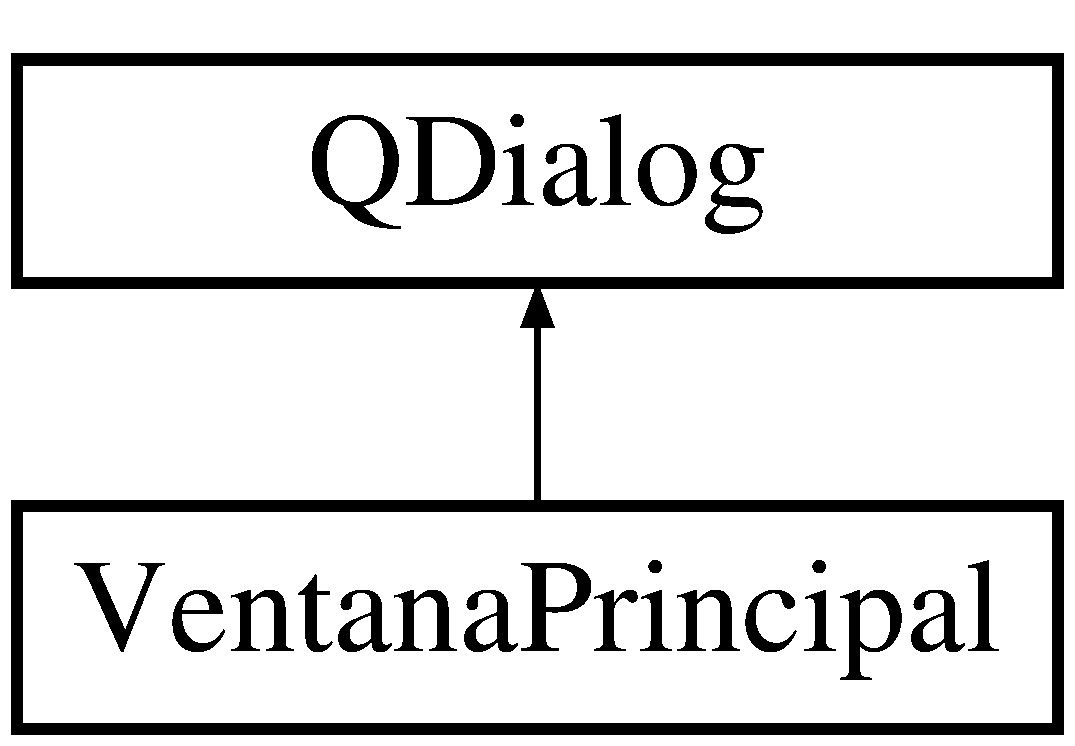
\includegraphics[height=2.000000cm]{class_ventana_principal}
\end{center}
\end{figure}
\subsection*{Public Slots}
\begin{DoxyCompactItemize}
\item 
\hypertarget{class_ventana_principal_a240d397814305d052a39d37f2790f763}{void {\bfseries on\-\_\-jugar\-\_\-clicked} ()}\label{class_ventana_principal_a240d397814305d052a39d37f2790f763}

\end{DoxyCompactItemize}
\subsection*{Signals}
\begin{DoxyCompactItemize}
\item 
\hypertarget{class_ventana_principal_ae9a4442771ee97d0335afa47c7d6a63b}{void {\bfseries avisojugar} (bool f)}\label{class_ventana_principal_ae9a4442771ee97d0335afa47c7d6a63b}

\end{DoxyCompactItemize}
\subsection*{Public Member Functions}
\begin{DoxyCompactItemize}
\item 
\hypertarget{class_ventana_principal_afc1895e635aa9cae6c2890882727f12b}{{\bfseries Ventana\-Principal} (Q\-Widget $\ast$parent=0)}\label{class_ventana_principal_afc1895e635aa9cae6c2890882727f12b}

\end{DoxyCompactItemize}


The documentation for this class was generated from the following files\-:\begin{DoxyCompactItemize}
\item 
\hyperlink{ventanaprincipal_8h}{ventanaprincipal.\-h}\item 
ventanaprincipal.\-cpp\end{DoxyCompactItemize}

\chapter{File Documentation}
\hypertarget{acercade_8h}{\section{acercade.\-h File Reference}
\label{acercade_8h}\index{acercade.\-h@{acercade.\-h}}
}


contiene una descripcion sobre los creadores del juego.  


{\ttfamily \#include $<$Q\-Dialog$>$}\\*
\subsection*{Classes}
\begin{DoxyCompactItemize}
\item 
class \hyperlink{classacercade}{acercade}
\end{DoxyCompactItemize}


\subsection{Detailed Description}
contiene una descripcion sobre los creadores del juego. \begin{DoxyAuthor}{Author}
Luis Caviedes 

Luis Vasquez
\end{DoxyAuthor}
\begin{DoxyDate}{Date}
07/07/2013 
\end{DoxyDate}

\hypertarget{eleccion_8h}{\section{eleccion.\-h File Reference}
\label{eleccion_8h}\index{eleccion.\-h@{eleccion.\-h}}
}


Este archivo contiene la definicion de los slots para el comienzo del juego.  


{\ttfamily \#include $<$Q\-Dialog$>$}\\*
\subsection*{Classes}
\begin{DoxyCompactItemize}
\item 
class \hyperlink{classeleccion}{eleccion}
\end{DoxyCompactItemize}


\subsection{Detailed Description}
Este archivo contiene la definicion de los slots para el comienzo del juego. \begin{DoxyAuthor}{Author}
Luis Caviedes 

Luis Vasquez
\end{DoxyAuthor}
\begin{DoxyDate}{Date}
07/07/2013 
\end{DoxyDate}

\hypertarget{instrucciones_8h}{\section{instrucciones.\-h File Reference}
\label{instrucciones_8h}\index{instrucciones.\-h@{instrucciones.\-h}}
}


contiene una breve explicación de la jugabilidad del sudoku.  


{\ttfamily \#include $<$Q\-Dialog$>$}\\*
\subsection*{Classes}
\begin{DoxyCompactItemize}
\item 
class \hyperlink{classinstrucciones}{instrucciones}
\end{DoxyCompactItemize}


\subsection{Detailed Description}
contiene una breve explicación de la jugabilidad del sudoku. \begin{DoxyAuthor}{Author}
Luis Caviedes 

Luis Vasquez
\end{DoxyAuthor}
\begin{DoxyDate}{Date}
07/07/2013 
\end{DoxyDate}

\hypertarget{jugador_8h}{\section{jugador.\-h File Reference}
\label{jugador_8h}\index{jugador.\-h@{jugador.\-h}}
}


contiene la declaracion del tipo de datos jugador y sus respectivos getter y setter.  


{\ttfamily \#include $<$Q\-String$>$}\\*
\subsection*{Classes}
\begin{DoxyCompactItemize}
\item 
class \hyperlink{class_jugador}{Jugador}
\end{DoxyCompactItemize}


\subsection{Detailed Description}
contiene la declaracion del tipo de datos jugador y sus respectivos getter y setter. \begin{DoxyAuthor}{Author}
Luis Caviedes 

Luis Vasquez
\end{DoxyAuthor}
\begin{DoxyDate}{Date}
07/07/2013 
\end{DoxyDate}

\hypertarget{lcdnumber_8h}{\section{lcdnumber.\-h File Reference}
\label{lcdnumber_8h}\index{lcdnumber.\-h@{lcdnumber.\-h}}
}


contiene la definicion del cronometro utilizado en la interfaz del sudoku.  


{\ttfamily \#include $<$Q\-L\-C\-D\-Number$>$}\\*
{\ttfamily \#include $<$Qt\-Gui$>$}\\*
\subsection*{Classes}
\begin{DoxyCompactItemize}
\item 
class \hyperlink{class_l_c_d_number}{L\-C\-D\-Number}
\end{DoxyCompactItemize}


\subsection{Detailed Description}
contiene la definicion del cronometro utilizado en la interfaz del sudoku. \begin{DoxyAuthor}{Author}
Luis Caviedes 

Luis Vasquez
\end{DoxyAuthor}
\begin{DoxyDate}{Date}
07/07/2013 
\end{DoxyDate}

\hypertarget{ranking_8h}{\section{ranking.\-h File Reference}
\label{ranking_8h}\index{ranking.\-h@{ranking.\-h}}
}


presentacion de los jugadores que han terminado el sudoku de manera satisfactoria.  


{\ttfamily \#include $<$Q\-Dialog$>$}\\*
{\ttfamily \#include $<$Qt\-Gui$>$}\\*
{\ttfamily \#include \char`\"{}jugador.\-h\char`\"{}}\\*
\subsection*{Classes}
\begin{DoxyCompactItemize}
\item 
class \hyperlink{class_ranking}{Ranking}
\end{DoxyCompactItemize}


\subsection{Detailed Description}
presentacion de los jugadores que han terminado el sudoku de manera satisfactoria. \begin{DoxyAuthor}{Author}
Luis Caviedes 

Luis Vasquez
\end{DoxyAuthor}
\begin{DoxyDate}{Date}
07/07/2013 
\end{DoxyDate}

\hypertarget{sudoku_8h}{\section{sudoku.\-h File Reference}
\label{sudoku_8h}\index{sudoku.\-h@{sudoku.\-h}}
}


Este archivo contiene la definicion de las funciones para el la creación, validación y presentación del sudoku. ademas permite cargar y guardar la partida.  


{\ttfamily \#include $<$Q\-Main\-Window$>$}\\*
{\ttfamily \#include $<$Q\-Line\-Edit$>$}\\*
{\ttfamily \#include $<$Q\-Grid\-Layout$>$}\\*
{\ttfamily \#include $<$Q\-File$>$}\\*
{\ttfamily \#include $<$string$>$}\\*
{\ttfamily \#include \char`\"{}lcdnumber.\-h\char`\"{}}\\*
{\ttfamily \#include $<$Q\-String$>$}\\*
{\ttfamily \#include \char`\"{}jugador.\-h\char`\"{}}\\*
\subsection*{Classes}
\begin{DoxyCompactItemize}
\item 
class \hyperlink{classsudoku}{sudoku}
\end{DoxyCompactItemize}


\subsection{Detailed Description}
Este archivo contiene la definicion de las funciones para el la creación, validación y presentación del sudoku. ademas permite cargar y guardar la partida. \begin{DoxyAuthor}{Author}
Luis Caviedes 

Luis Vasquez
\end{DoxyAuthor}
\begin{DoxyDate}{Date}
07/07/2013 
\end{DoxyDate}

\hypertarget{ventanaprincipal_8h}{\section{ventanaprincipal.\-h File Reference}
\label{ventanaprincipal_8h}\index{ventanaprincipal.\-h@{ventanaprincipal.\-h}}
}


ventana principal del juego Sudoku.  


{\ttfamily \#include $<$Q\-Dialog$>$}\\*
\subsection*{Classes}
\begin{DoxyCompactItemize}
\item 
class \hyperlink{class_ventana_principal}{Ventana\-Principal}
\end{DoxyCompactItemize}


\subsection{Detailed Description}
ventana principal del juego Sudoku. \begin{DoxyAuthor}{Author}
Luis Caviedes 

Luis Vasquez
\end{DoxyAuthor}
\begin{DoxyDate}{Date}
07/07/2013 
\end{DoxyDate}

%--- End generated contents ---

% Index
\newpage
\phantomsection
\addcontentsline{toc}{part}{Index}
\printindex

\end{document}
